\documentclass [11pt,twoside]{article}
\usepackage[utf8]{inputenc}
\usepackage[T1]{fontenc}

%Page margins, header and footer positions
\usepackage{geometry}
 \geometry{
 a4paper,
 total={210mm,297mm},
 left=25mm,
 right=25mm,
 top=30mm,
 bottom=25mm,
 headsep=7mm}

\interfootnotelinepenalty=10000

%To display filling dots in the TOC for all entries
\usepackage[titles]{tocloft}
\renewcommand{\cftsecleader}{\cftdotfill{\cftdotsep}}

%Define new header and footer style
\usepackage{fancyhdr}

\pagestyle{fancy}
\fancyhf{}
\lhead{\color{Gray}{\small{Best Bike Paths project by Umme Humaira Himi, Ahmed Hassan, Shuvro Ahmed}}}
\lfoot{\textcolor{Gray}{\small{Copyright © 2025, Umme Humaira Himi, Ahmed Hassan, Shuvro Ahmed – All rights reserved}}}
\rfoot{\textcolor{Gray}{\thepage}}
\renewcommand{\headrulewidth}{0pt}

%PACKAGES
\usepackage{wasysym}
\usepackage{pifont}

\newcommand{\supported}{\ding{52}\xspace}
\newcommand{\unsupported}{\ding{55}\xspace}
\newcommand{\partsupported}{\textcolor{black!40}{\ding{52}}\xspace}
\newcommand{\lowsupported}{\textcolor{black!20}{\ding{52}}\xspace}
\newcommand{\unknowsupported}{\textbf{?}\xspace}

%Font: Times
\usepackage{times}
%Change monospaced font
\renewcommand{\ttdefault}{lmtt}

%tables
\usepackage{tabu}
\usepackage{tabularx}
\usepackage{ltablex}
\usepackage{longtable}
\usepackage{float} % To allow the use of H modifier in long tables

%landscape mode
\usepackage{pdflscape}
\usepackage{rotating}
\usepackage{caption}

%make landscape mode be sensitive to even and odd pages
%start
\def\myrotate{\ifodd\c@page\else-\fi 90}
\makeatletter
\global\let\orig@begin@landscape=\landscape%
\global\let\orig@end@landscape=\endlandscape%
\gdef\@true{1}
\gdef\@false{0}
\gdef\landscape{%
    \global\let\within@landscape=\@true%
    \orig@begin@landscape%
}%
\gdef\endlandscape{%
    \orig@end@landscape%
    \global\let\within@landscape=\@false%
}%
\@ifpackageloaded{pdflscape}{%
    \gdef\pdf@landscape@rotate{\PLS@Rotate}%
}{
    \gdef\pdf@landscape@rotate#1{}%
}
\let\latex@outputpage\@outputpage
\def\@outputpage{
    \ifx\within@landscape\@true%
        \if@twoside%
            \ifodd\c@page%
                \gdef\LS@rot{\setbox\@outputbox\vbox{%
                    \pdf@landscape@rotate{-90}%
                    \hbox{\rotatebox{90}{\hbox{\rotatebox{180}{\box\@outputbox}}}}}%
                }%
            \else%
                \gdef\LS@rot{\setbox\@outputbox\vbox{%
                    \pdf@landscape@rotate{+90}%
                    \hbox{\rotatebox{90}{\hbox{\rotatebox{0}{\box\@outputbox}}}}}%
                }%
            \fi%
        \else%
            \gdef\LS@rot{\setbox\@outputbox\vbox{%
                \pdf@landscape@rotate{+90}%
                \hbox{\rotatebox{90}{\hbox{\rotatebox{0}{\box\@outputbox}}}}}%
            }%
        \fi%
    \fi%
    \latex@outputpage%
}
\makeatother
%end

%graphics
\usepackage{graphicx}
\usepackage[dvipsnames, table]{xcolor}
%If you upload images from PC, you need to insert code for the path here (different for Windows and Unix OS)

%References
%\usepackage{xpatch}
%\usepackage[backend=biber, style=numeric, citestyle=numeric, sorting=none]{biblatex}
%\addbibresource{main.bib}

%Other
\usepackage{ifthen}
\usepackage{xspace}
\usepackage{enumitem}
\usepackage{amssymb}
\usepackage[pdftex, colorlinks]{hyperref}
\newcommand{\comment}[1]{{\color{Red}$\blacktriangleright$ Comment: #1 $\blacktriangleleft$}}


% Some utilities\ldots
\usepackage{soul}
\usepackage{tikz}

\usetikzlibrary{calc}
\usetikzlibrary{decorations.pathmorphing}


\makeatletter

\newcommand{\defhighlighter}[3][]{%
  \tikzset{every highlighter/.style={color=#2, fill opacity=#3, #1}}%
}

\defhighlighter{yellow}{.5}

\newcommand{\highlight@DoHighlight}{
  \fill [ decoration = {random steps, amplitude=1pt, segment length=15pt}
        , outer sep = -15pt, inner sep = 0pt, decorate
       , every highlighter, this highlighter ]
        ($(begin highlight)+(0,8pt)$) rectangle ($(end highlight)+(0,-3pt)$) ;
}

\newcommand{\highlight@BeginHighlight}{
  \coordinate (begin highlight) at (0,0) ;
}

\newcommand{\highlight@EndHighlight}{
  \coordinate (end highlight) at (0,0) ;
}

\newdimen\highlight@previous
\newdimen\highlight@current

\DeclareRobustCommand*\highlight[1][]{%
  \tikzset{this highlighter/.style={#1}}%
  \SOUL@setup
  %
  \def\SOUL@preamble{%
    \begin{tikzpicture}[overlay, remember picture]
      \highlight@BeginHighlight
      \highlight@EndHighlight
    \end{tikzpicture}%
  }%
  %
  \def\SOUL@postamble{%
    \begin{tikzpicture}[overlay, remember picture]
      \highlight@EndHighlight
      \highlight@DoHighlight
    \end{tikzpicture}%
  }%
  %
  \def\SOUL@everyhyphen{%
    \discretionary{%
      \SOUL@setkern\SOUL@hyphkern
      \SOUL@sethyphenchar
      \tikz[overlay, remember picture] \highlight@EndHighlight ;%
    }{%
    }{%
      \SOUL@setkern\SOUL@charkern
    }%
  }%
  %
  \def\SOUL@everyexhyphen##1{%
    \SOUL@setkern\SOUL@hyphkern
    \hbox{##1}%
    \discretionary{%
      \tikz[overlay, remember picture] \highlight@EndHighlight ;%
    }{%
    }{%
      \SOUL@setkern\SOUL@charkern
    }%
  }%
  %
  \def\SOUL@everysyllable{%
    \begin{tikzpicture}[overlay, remember picture]
      \path let \p0 = (begin highlight), \p1 = (0,0) in \pgfextra
        \global\highlight@previous=\y0
        \global\highlight@current =\y1
      \endpgfextra (0,0) ;
      \ifdim\highlight@current < \highlight@previous
        \highlight@DoHighlight
        \highlight@BeginHighlight
      \fi
    \end{tikzpicture}%
    \the\SOUL@syllable
    \tikz[overlay, remember picture] \highlight@EndHighlight ;%
  }%
  \SOUL@
}

\makeatother

% Common abbrev. are set as commands to ensure proper spacing after the dot
\RequirePackage{xspace}
\newcommand{\ie}{i.e.\@\xspace}
\newcommand{\aka}{a.k.a.\@\xspace}
\newcommand{\Ie}{I.e.\@\xspace}
\newcommand{\cf}{cf.\@\xspace}
\newcommand{\Cf}{Cf.\@\xspace}
\newcommand{\eg}{e.g.\@\xspace}
\newcommand{\Eg}{E.g.\@\xspace}
\newcommand{\etal}{et al.\@\xspace}
\newcommand{\etc}{etc.\@\xspace}
\newcommand{\wrt}{w.r.t.\@\xspace}
\newcommand{\Wrt}{W.r.t.\@\xspace}



\date{}


\begin{document}

%TITLE PAGE

\begin{titlepage}


%LOGO

\begin{table}[t!]
\centering
\rule{\textwidth}{0.6pt}
\vspace{0.6em}
\begin{minipage}[c]{0.68\textwidth}
    \raggedright%
    	{\textcolor{gray}{\large\bfseries Project by\\[0.35em] Shuvro Ahmed\\ Umme Humaira Himi\\ Ahmed Hassan}}
\end{minipage}\hfill
\begin{minipage}[c]{0.30\textwidth}
    \centering
    \vspace{0pt}% ensure vertical centering within the rules
    
\includegraphics[width=\linewidth]{Images/PolimiLogo}
\end{minipage}
\vspace{0.6em}
\rule{\textwidth}{0.6pt}
\end{table}
\vspace{7cm}
%TITLE 
\begin{center}
    \vspace*{1cm}

    \rule{\textwidth}{0.8pt}\\[0.8cm]

    {\bfseries\Huge
        Requirement Analysis and\\[0.2em]
        Specification Document}\\[0.6cm]

    {\large\bfseries for}\\[0.6cm]

    {\bfseries\LARGE
        Best Bike Paths}\\[0.8cm]

    \rule{0.6\textwidth}{0.8pt}\\[0.6cm]

    {\small \textit{Politecnico di Milano – A.Y. 2025/2026}}

\end{center}

\vfill
\begin{table}[h!]
\begin{tabularx}{\textwidth}{@{}>{\raggedright\arraybackslash}p{0.3\textwidth}>{\raggedright\arraybackslash}X@{}}
\toprule
	\textbf{Deliverable:} & DD \\
	\textbf{Title:} & Design document \\
	\textbf{Authors:} & Shuvro Ahmed, Umme Humaira Himi, Ahmed Hassan \\
	\textbf{Version:} & 1.0 \\
	\textbf{Date:} & 7-January-2026 \\
	\textbf{Download page:} & \url{https://github.com/H-I-M-I/HassanAhmedHimi} \\
	\textbf{Copyright:} & {\small Copyright \textcopyright{} 2025, Shuvro Ahmed, Umme Humaira Himi, Ahmed Hassan – All rights reserved} \\
\bottomrule
\end{tabularx}
\end{table}

\end{titlepage}

%Define deliverable specific info
%Replace cell contents where needed
\begin{table}[h!]
\begin{tabu} to \textwidth { X[0.3,r,p] X[0.7,l,p] }
\hline

\textbf{Deliverable:} & RASD\\
\textbf{Title:} & Requirement Analysis and Verification Document \\
\textbf{Authors:} & YOUR NAMES \\
\textbf{Version:} & 1.0 \\ 
\textbf{Date:} & 31-January-2016 \\
\textbf{Download page:} & LINK TO YOUR REPOSITORY \\
\textbf{Copyright:} & Copyright © 2017, YOUR NAMES – All rights reserved \\
\hline
\end{tabu}
\end{table}




\setcounter{page}{2}


%------------------------------------------------------------------------------------------------------------------------------------------------
\newpage
\addcontentsline{toc}{section}{Table of Contents}
\tableofcontents
\newpage
\addcontentsline{toc}{section}{List of Figures}
\listoffigures
\addcontentsline{toc}{section}{List of Tables}
\listoftables

%------------------------------------------------------------------------------------------------------------------------------------------------
\clearpage
{\color{Blue}{\section{Introduction}}}
\label{sect:introduction}
\subsection{Purpose}

The Best Bike Paths (BBP) system is intended to assist bicycle riders in determining and using the best available bike path given a city's context including factors such as path safety, user-friendly design, obstacles etc.
Users can provide information about the bike path by logging trips or manually and automatically reporting obstacles faced during cycling.
The objective of this Design Document is to show the structure of BBP system in order meet these goal, report about architectural organization and design decisions which have been made to ensure functionalities described in Requirement Analysis and Specification Document (RASD).
The aim of this paper is to be a detailed specification for developers and testers in following phases as implementation, integration and testing phase.

\subsection{Scope}

The BBP system collects, administers and displays bike path and cycling information. More specifically, the system allows for the capturing of bike trips, its includes and validating path-related information, and generating optimal bike paths between any two points based on an aggregated user's input.
This Design Document proposes how the software architecture should be, and what components are necessary to implement these functionalities, its interactions and their interfaces.
This is intended to provide a clear reference for developers and testers during the subsequent phases of implementation, integration, and testing.

\subsection{Definitions}

This subsection reports the definitions of the main concepts used throughout this Design Document. Additional definitions introduced during the requirements analysis phase are described in the RASD.

\begin{itemize}
    \item \textbf{Bike Path}: A path suitable for cycling, either because it includes a dedicated bike lane or because car traffic is limited and compatible with bicycle usage.
    \item \textbf{Trip}: A cycling activity recorded by a registered user, consisting of spatial and temporal data collected during movement.
    \item \textbf{Publishable Information}: Information about bike paths or obstacles that has been confirmed by the user and made visible to the community.
\end{itemize}

\subsection{Acronyms}

\begin{itemize}
    \item \textbf{BBP}: Best Bike Paths
    \item \textbf{DD}: Design Document
    \item \textbf{RASD}: Requirement Analysis and Specification Document
    \item \textbf{UI}: User Interface
    \item \textbf{API}: Application Programming Interface
\end{itemize}

\subsection{Abbreviations}

\begin{itemize}
    \item \textbf{GPS}: Global Positioning System
    \item \textbf{DB}: Database
\end{itemize}

\subsection{Revision History}

Version 1.0 : 07/01/2026.

\subsection{Reference Documents}

This subsection lists the documents that have been consulted and referenced during the preparation of this Design Document and that provide the basis for the architectural and design choices described in the following sections.

\begin{itemize}
    \item Requirement Analysis and Specification Document (RASD) - Best Bike Paths
    \item Software Engineering 2 - Assignment R\&DD, A.Y. 2025--2026
    \item Software Engineering 2 course material and lecture slides
\end{itemize}

\subsection{Document Structure}

This document is structured as follows:

\begin{enumerate}
    \item \textbf{Introduction}: provides a brief description of the project, focusing on the motivations and goals to be achieved through its development, as defined in the RASD.
    \item \textbf{Architectural Design}: describes the architecture of the system at different levels of granularity, including the main components, their interactions, and the adopted architectural patterns.
    \item \textbf{User Interface Design}: presents the organization of the user interface of the platform and describes how users interact with the system.
    \item \textbf{Requirements Traceability}: explains how the requirements defined in the RASD are satisfied by the design elements introduced in this document.
    \item \textbf{Implementation, Integration and Test Plan}: provides an overview of the implementation strategy, integration activities, and testing approach adopted for the system.
    \item \textbf{Effort Spent}: reports the effort spent by each group member in the preparation of this document.
    \item \textbf{Bibliography}: contains the references to the documents and tools used to produce this Design Document.
\end{enumerate}



%------------------------------------------------------------------------------------------------------------------------------------------------
\clearpage
{\color{Blue}{\section{Overall Description}}}
\label{sect:overview}
Here you can see how to include an image in your document.

\begin{sidewaysfigure}
\centering
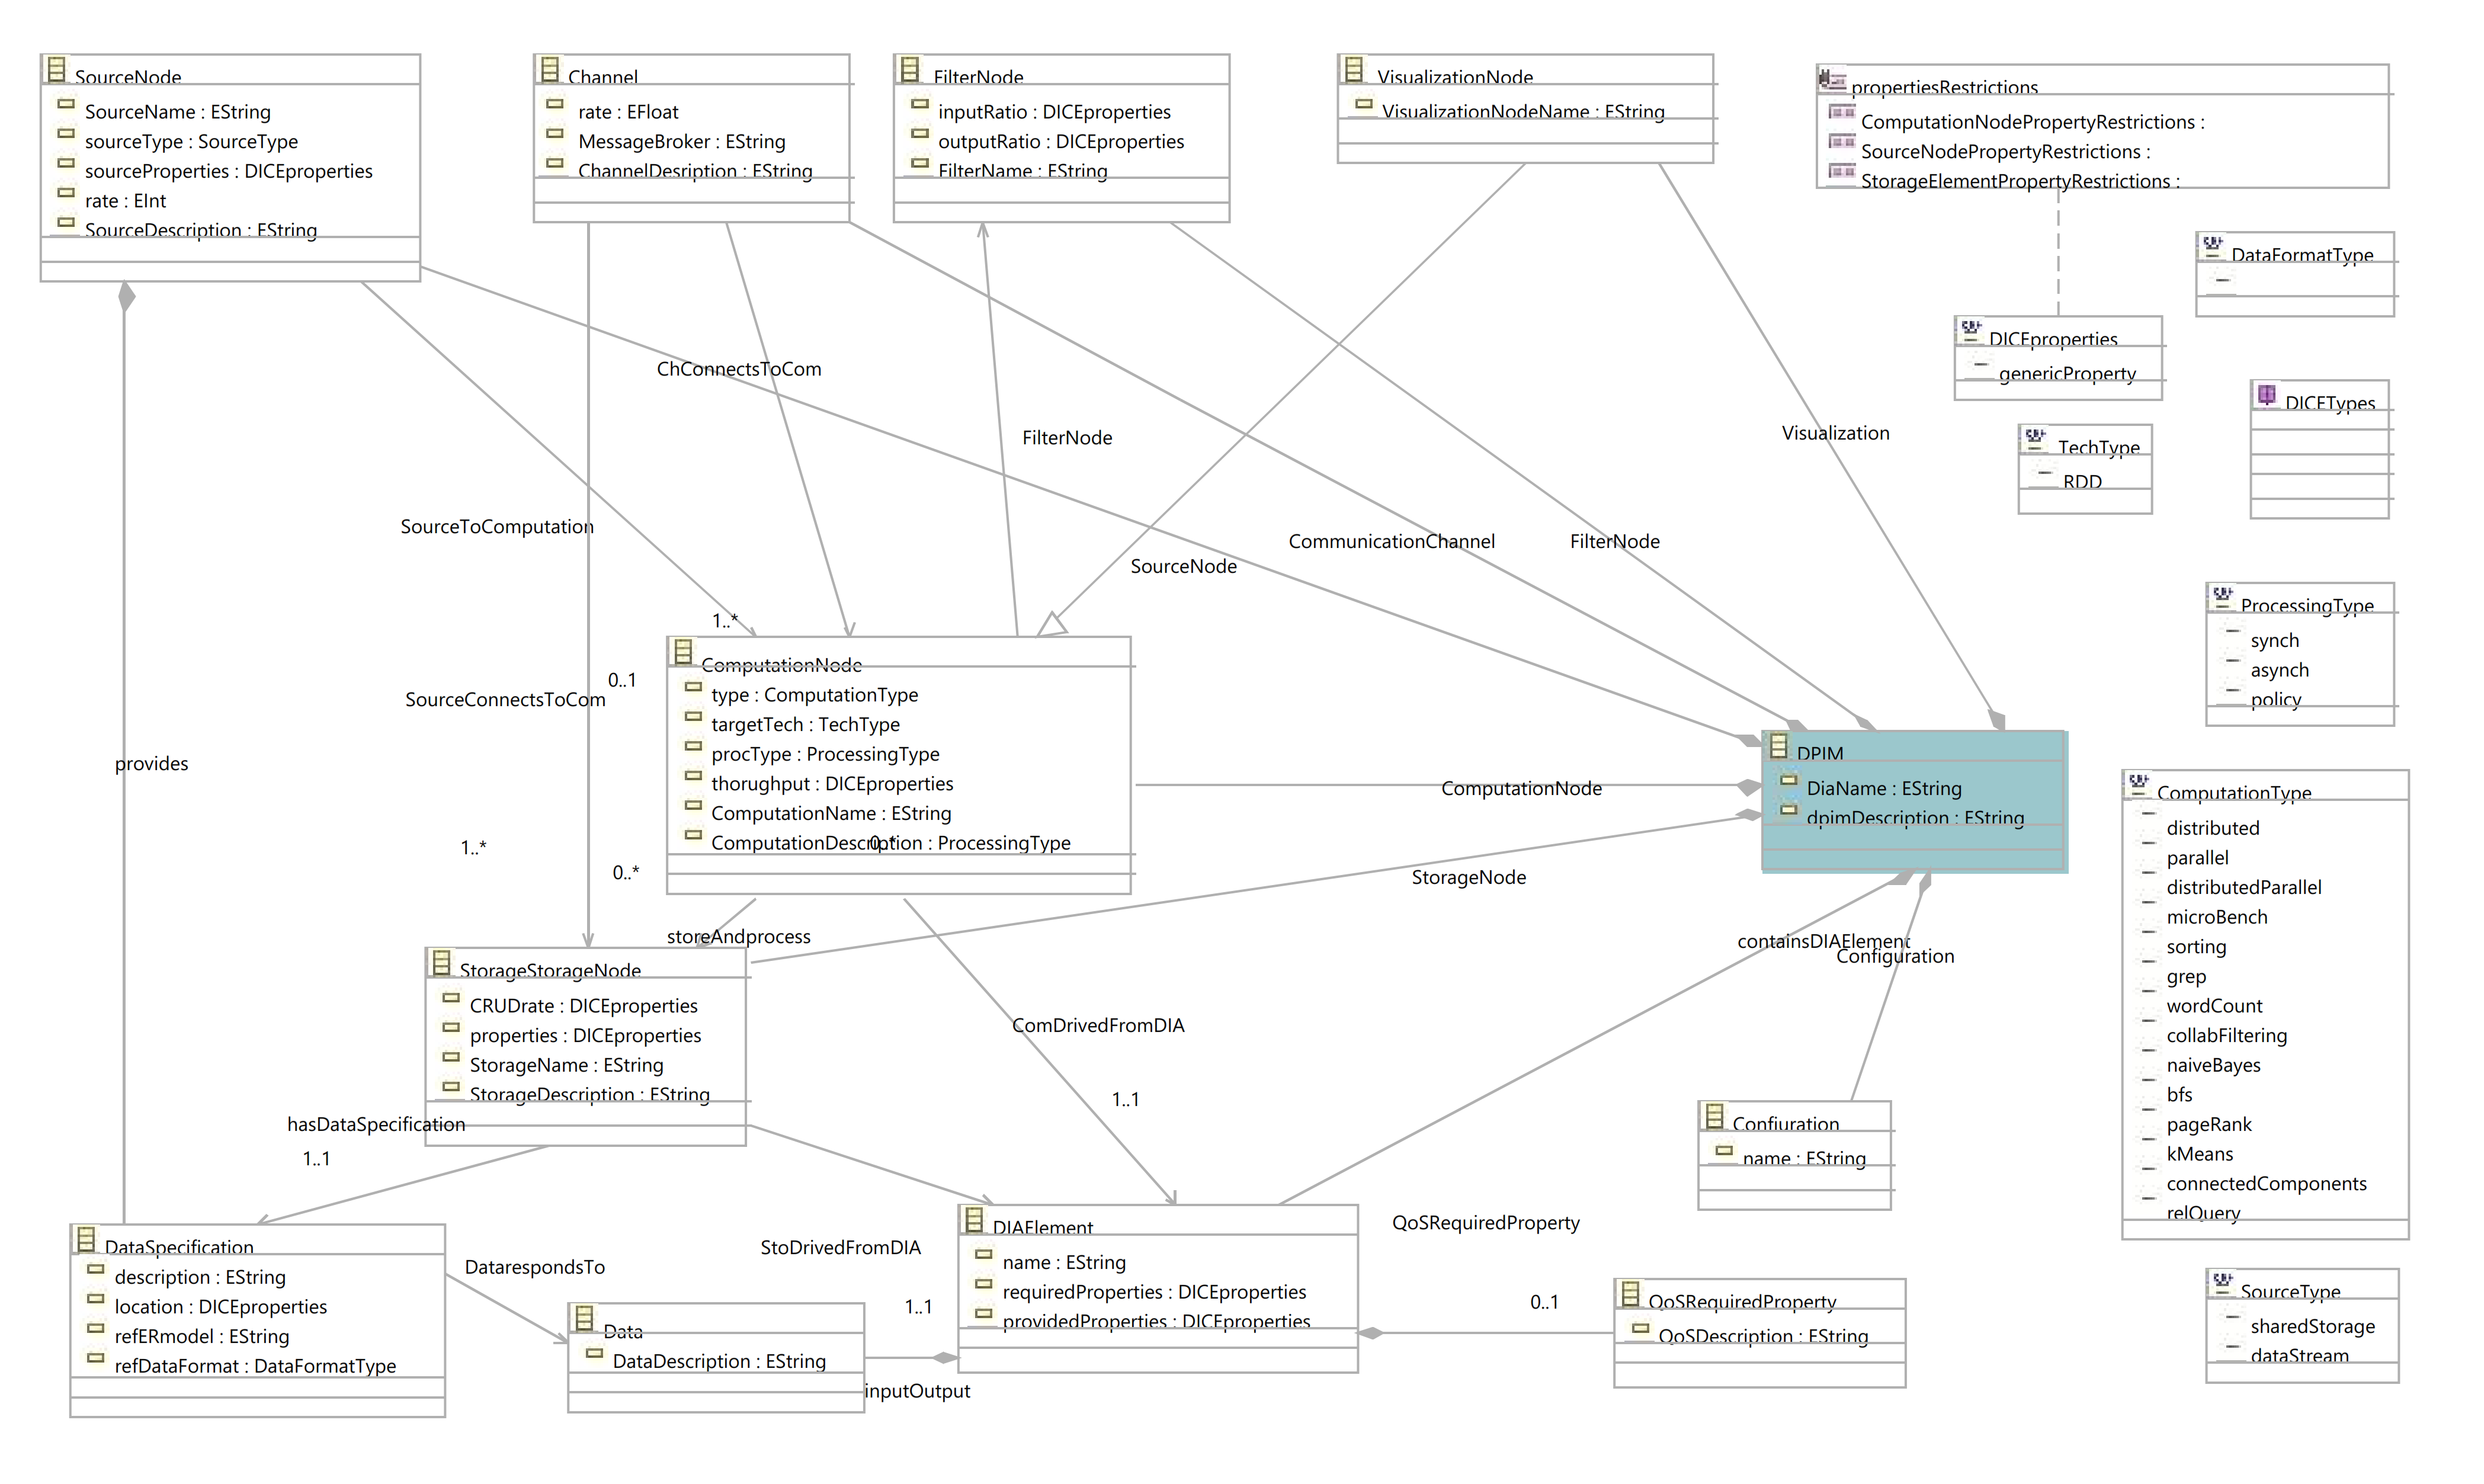
\includegraphics[width=\textwidth]{Images/11.png}
\caption{\label{fig:metamodel}DICE DPIM metamodel.}
\end{sidewaysfigure}

\begin{figure}
\centering
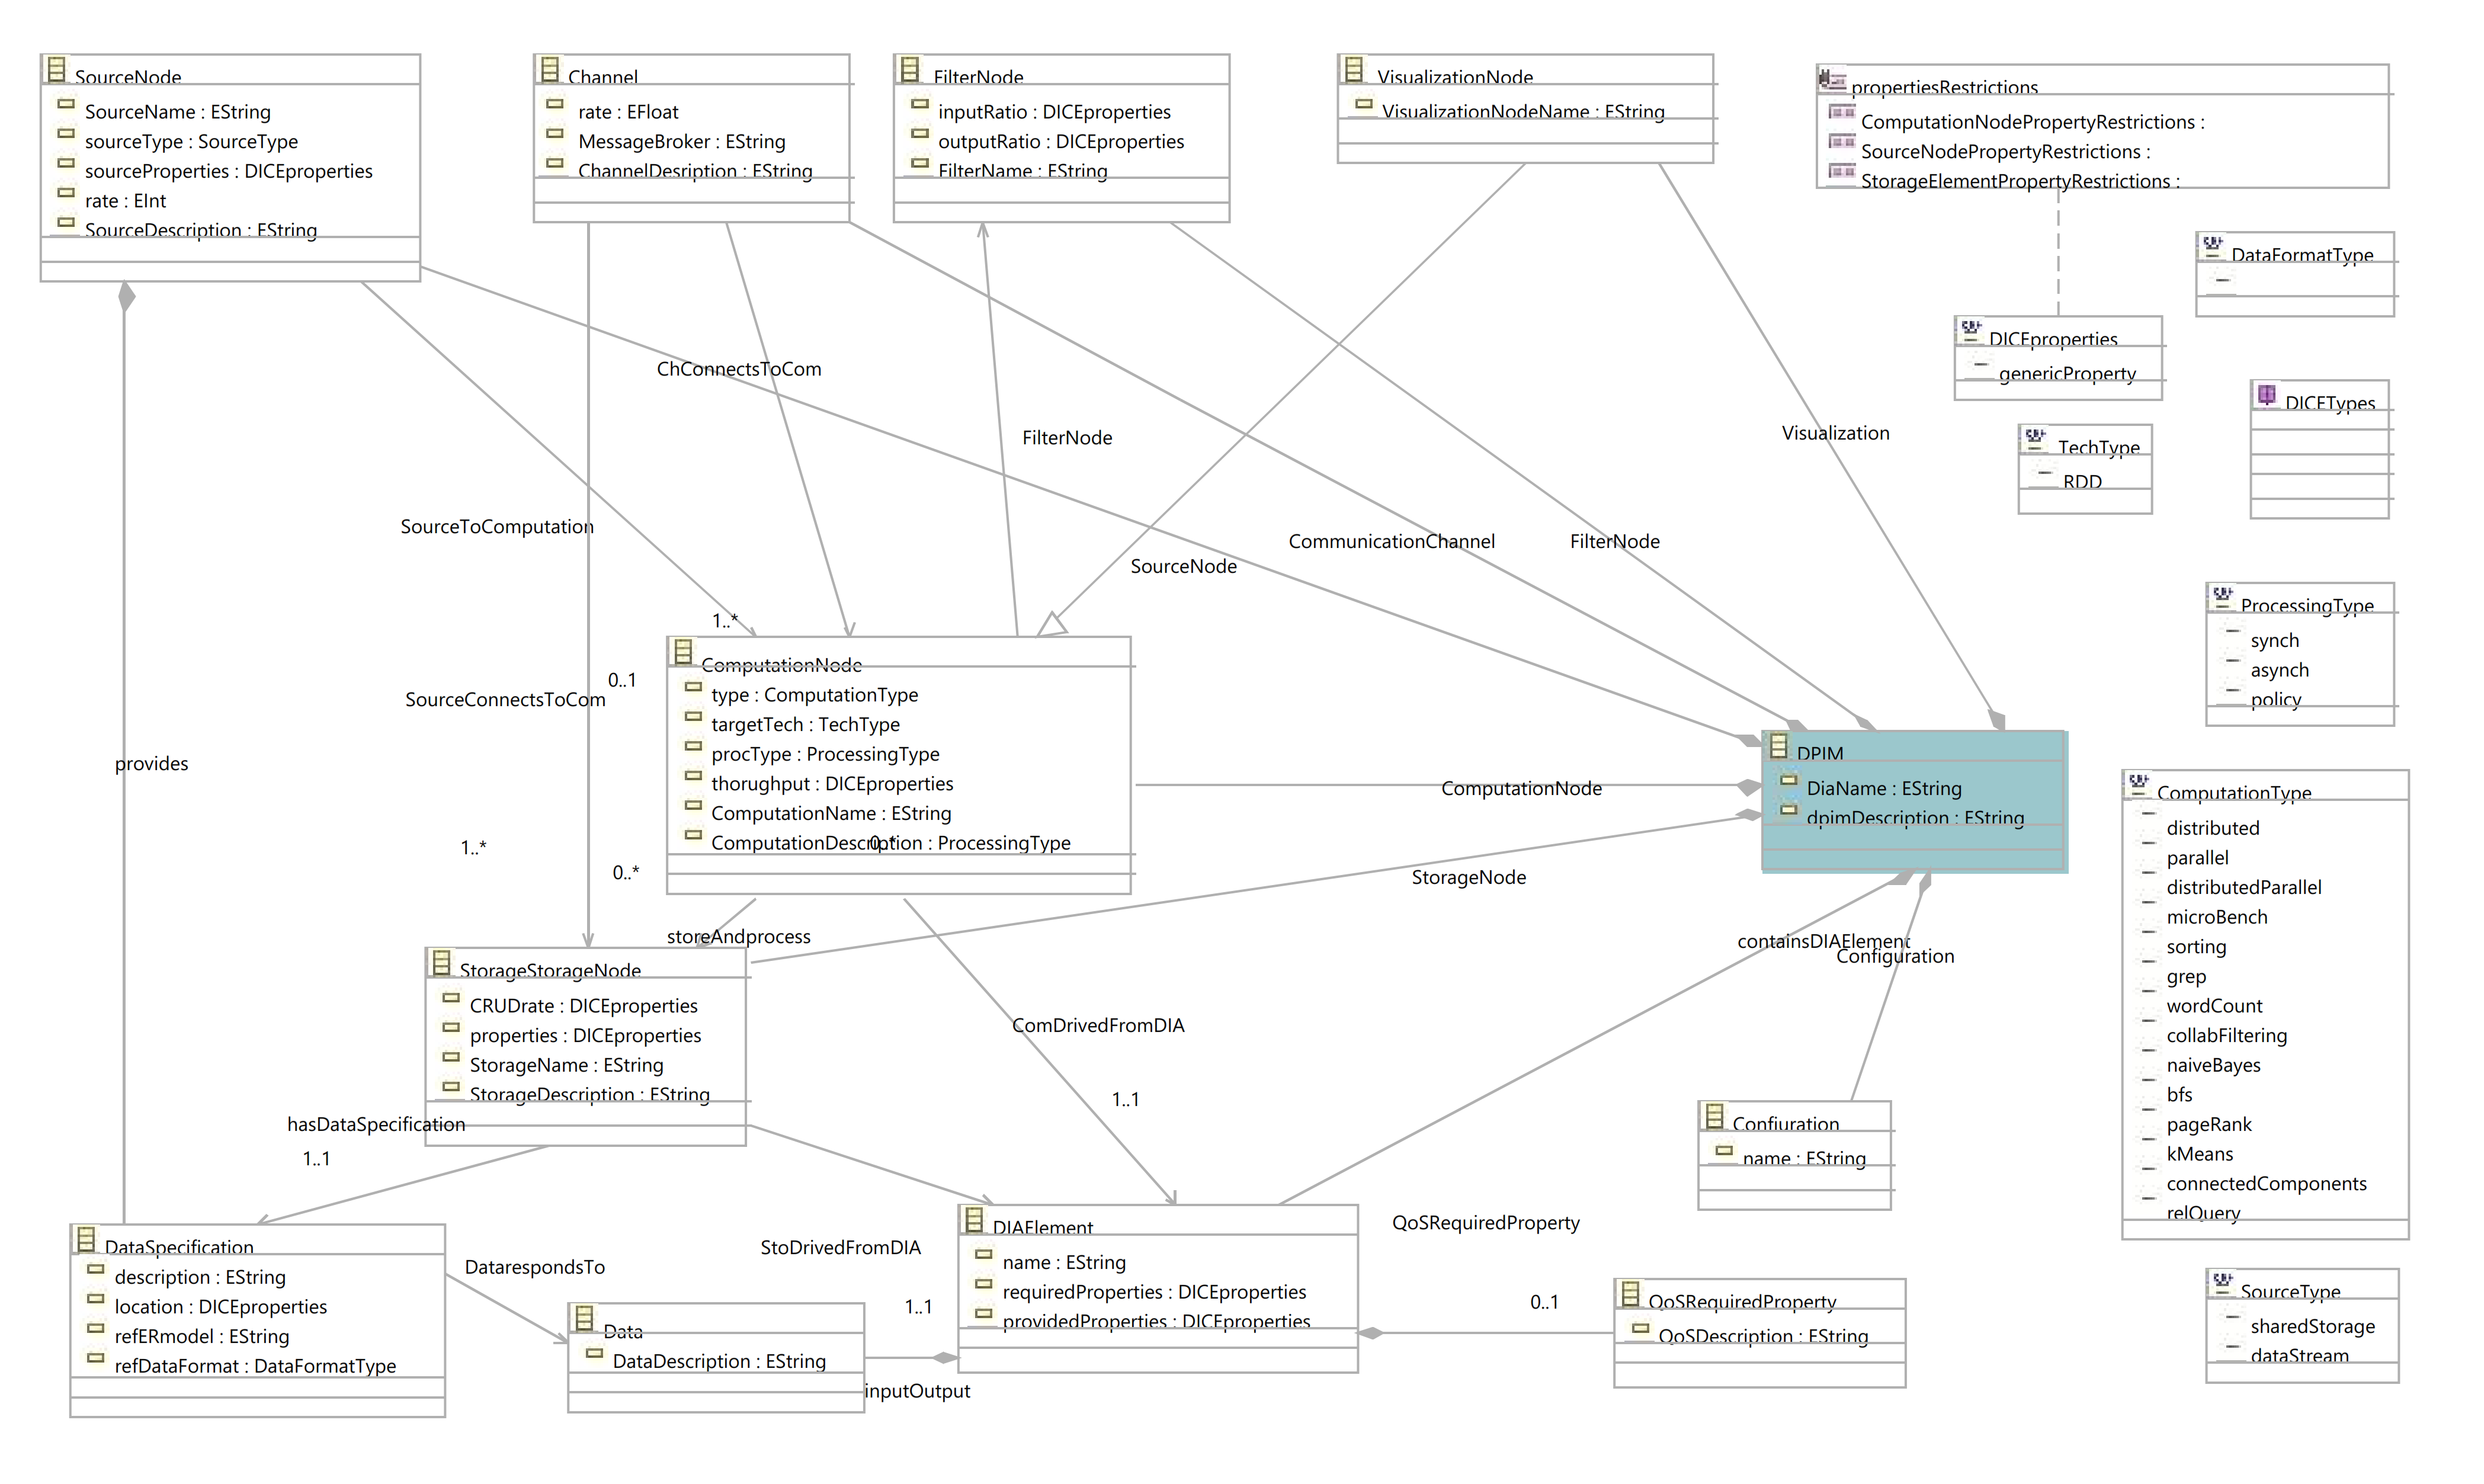
\includegraphics[width=\textwidth]{Images/11.png}
\caption{\label{fig:metamodel2}DICE DPIM metamodel in portrait form.}
\end{figure}

Here is the command to refer to another element (section, figure, table, ...) in the document: \emph{As discussed in Section~\ref{sect:overview} and as shown in Figure~\ref{fig:metamodel}, ...}. Here is how to introduce a bibliographic citation~\cite{DAM}. Bibliographic references should be included in a \texttt{.bib} file. 

Table generation is a bit complicated in Latex. You will soon become proficient, but to start you can rely on tools or external services. See for instance this \href{https://www.tablesgenerator.com}{https://www.tablesgenerator.com}. 


%------------------------------------------------------------------------------------------------------------------------------------------------
\clearpage
{\color{Blue}{\section{Specific Requirements}}}
\label{sect:requirements}
Organize this section according to the rules defined in the project description. 


%------------------------------------------------------------------------------------------------------------------------------------------------
\clearpage
{\color{Blue}{\section{Formal Analysis Using Alloy}}}
\label{sect:alloy}
Organize this section according to the rules defined in the project description. 


%------------------------------------------------------------------------------------------------------------------------------------------------
\clearpage
{\color{Blue}{\section{Effort Spent}}}
\label{sect:effort}
\subsection{Shuvro Ahmed}

{\centering
\begin{tabular}{@{}p{8cm}c@{}}
	\toprule
	\textbf{Task} & \textbf{Hours} \\
\midrule
Design Document structure setup & 1 \\
Architectural overview review and alignment with RASD & 2 \\
Deployment View – design and refinement & 5 \\
Deployment View description and node explanations & 2 \\
Runtime View – UC5/UC6 Path Search & 4 \\
Runtime View – UC1 Record Trip + Weather Enrichment & 4 \\
Runtime View – UC3 Manual Path Contribution & 3 \\
Runtime View – UC4 Automatic Detection + User Confirmation & 5 \\
Runtime View – Aggregation and Conflict Resolution (G5/F6) & 3 \\
Component Interfaces – interface identification and consolidation & 3 \\
Component Interfaces – final bullet-style interface specification & 2 \\
Consistency checks between RASD and DD (goals, use cases, services) & 2 \\
Fix LaTeX issues, figures, and repository organization & 3 \\
\bottomrule
\end{tabular}\par}



%------------------------------------------------------------------------------------------------------------------------------------------------
\clearpage
\addcontentsline{toc}{section}{References}
\bibliographystyle{plain}
\bibliography{main}
%------------------------------------------------------------------------------------------------------------------------------------------------




\end{document}
